\chapter{Methodology}\label{chapter:methodology}


% NOTE: add HMM as baseline

This work aims to construct a graph neural network-based architecture for predicting, analyzing, and detecting any potentially abnormal behavior regarding the driver during the whole driving process. In particular, The model extracts a description graph, the so-called scene graph, of the driver from the video filmed inside the vehicle and trains itself with these data to learn for future behavior prediction. The result will be used to compare and detect any abnormal behavior. Here we would lay most emphasis on the construction of the training model. To make precious anomaly detection we aim to predict not only if there is a behavior between humans and a specific kind of object but the type of behavior as well, which will cause several adaptions based on existing model \textit{JODIE}. 

This chapter will follow the pipeline of the whole work, as shown in figure \ref{fig:pipeline}. Progressively we would introduce the scene graph generation, the model architecture, and the training process. 

\begin{figure}
    \centering
    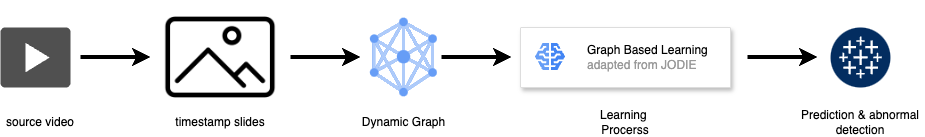
\includegraphics[width=\linewidth]{figures/04_pipeline.png}
    \caption{pipeline of the whole work}
    \label{fig:pipeline}
\end{figure}


\section{Scene graph generation}

The \textit{Drive \& Act} dataset comprises 12 hours of video data segmented into 29 lengthy sequences. For each sequence, we aim to generate a unique dynamic graph that temporally represents both the participant's actions and the relationships between objects observed in the video. This process involves several key steps.


First, by sliding through the video at intervals of $1/15$ second, we obtain a series of images. Theoretically, each image could yield a corresponding graph with the use of an object detection model \cite{tang2020unbiased}. Given that our objective is to predict driver behavior, we concentrate on the driver and the specific objects with which they interact. Consequently, we opt for a streamlined approach by directly extracting data from hierarchical labels within the dataset. A simplified example of these labels is presented in Table \ref{tab:hierarchical_labels}.

\clearpage

\begin{longtable}{ccccc}
    \toprule
    \textbf{file\_id} & \textbf{frame\_start} & \textbf{frame\_end} & \textbf{activity} & \textbf{chunk\_id} \\
    \midrule
    vp1/run1b.kinect\_color & 40 & 58 & standing\_by\_the\_door & 0 \\
    vp1/run1b.kinect\_color & 58 & 82 & closing\_door\_outside & 0 \\
    vp1/run1b.kinect\_color & 83 & 102 & standing\_by\_the\_door & 0 \\
    vp1/run1b.kinect\_color & 102 & 130 & opening\_door\_outside & 0 \\
    vp1/run1b.kinect\_color & 130 & 156 & entering\_car & 0 \\
    vp1/run1b.kinect\_color & 156 & 174 & closing\_door\_inside & 0 \\
    \bottomrule
    \caption{Example of the hierarchical labels Reproduced from\cite{9009583}}
    \label{tab:hierarchical_labels}
\end{longtable}


However, this table alone is insufficient for generating graphs, as it would require detecting objects at each individual timestamp to ensure data completeness. Instead, we construct the necessary dynamic graph by processing each timestamp sequentially: initially, we designate the participant as node \textbf{u} and relevant objects as nodes \textbf{v}. Then, by analyzing interactions at each timestamp, we add edges between the participant node and the relevant object nodes to reflect the associated actions. Unlike many traditional models, each edge is labeled with the specific activity being performed. The graph is updated with each subsequent timestamp, ultimately resulting in a dynamic graph that evolves along the temporal sequence.
    

Another key consideration in graph generation is the classification of activity labels. The raw dataset contains 39 distinct behaviors, which would be computationally intensive and overly too trivial to label directly. To address this, we employ \textbf{BART}, a denoising autoencoder designed for pretraining sequence-to-sequence models, to cluster these behaviors into four categories. This classification is based on whether the behavior is related to driving and whether it poses any potential risk, as our ultimate goal is to flag abnormal behaviors. The resulting behavior classifications are presented in Table \ref{tab:Behavior classification}.

\begin{figure}[h]
    \centering
    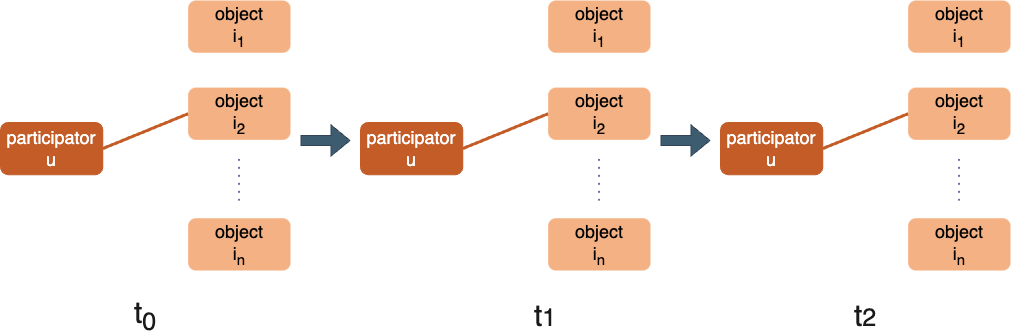
\includegraphics[width=\linewidth]{figures/04_DynamicGraph.png}
    \caption{Dynamic Graph Generation for Driver Behavior Recognition}
    \label{fig:DynamicGraph}
\end{figure}


% \clearpage

\begin{table}[h]
    \centering
    \begin{tabular}{ccp{10cm}}
        \toprule
        \textbf{No.} & \textbf{State} & \textbf{Behaviors} \\
        \midrule
        1 & \textbf{Driving concerned behaviors} & standing by the door, closing door outside, opening door outside, entering car, closing door inside, fastening seat belt, moving towards door, unfastening seat belt, opening door inside, exiting car \\
        \midrule
        2 & \textbf{Independent behaviors} & sitting still, looking or moving around (e.g. searching), looking back left shoulder, looking back right shoulder \\
        \midrule
        3 & \textbf{Eat or drink concerned behaviors} & preparing food, eating, opening bottle, drinking, closing bottle \\
        \midrule
        4 & \textbf{Other object concerned behaviors} & using multimedia display, sitting still, using multimedia display, pressing automation button, fetching an object, opening laptop, working on laptop, interacting with phone, closing laptop, placing an object, putting on jacket, taking off sunglasses, putting on sunglasses, reading newspaper, writing, talking on phone, reading magazine, taking off jacket, opening backpack, closing backpack, putting laptop into backpack, taking laptop from backpack \\
        \bottomrule
    \end{tabular}
    \caption{Behavior classification}
    \label{tab:Behavior classification}
\end{table}



Through the processes outlined above, all dynamic graphs have been successfully generated, as illustrated in Figure \ref{fig:DynamicGraph}. To streamline subsequent learning steps, these graphs are stored in a tabular format, as shown in Table \ref{tab:dynamic_graph_storage}.



\begin{table}[h]
    \centering
    \begin{tabular}{ccccc}
        \toprule
        \textbf{u} & \textbf{v} & \textbf{timestamp} & \textbf{state label} & \textbf{feature} \\
        \midrule
        1 & 2 & 127 & 0 & 0.27 \\
        \bottomrule
    \end{tabular}
    \caption{Storage of dynamic graph}
    \label{tab:dynamic_graph_storage}
\end{table}

As illustration of heads of this table is as following:

\begin{description}
    \item[u] The action initiator or generator, in our work typically representing the participant or driver.
    \item[v] The object or target that is acted upon or influenced by the action.
    \item[timestamp] The specific moment or time frame at which the action or interaction occurs.
    \item[stable label] A stable vector that characterizes the consistent attributes or categorical label associated with the edge.
    \item[feature] A weight vector representing the proportion of occurrences for a particular attribute (in this case, the location column), reflecting the relative frequency or appearance percentage of this attribute over time.
\end{description}


% we classify and label the behavior with LLM

\section{Baseline: Hidden Markov Model (HMM)}


The Hidden Markov Model (HMM) is a suitable baseline for our driver behavior prediction task due to its effectiveness in modeling temporal sequences with underlying hidden states, allowing it to capture the evolving patterns of driver behavior over time. HMMs provide a probabilistic framework that handles uncertainty in sequential data, making them a widely adopted baseline for tasks involving sequence prediction, including applications in graph neural network (GNN) models. In our work, this baseline serves as a foundation for comparison, particularly given that our hybrid model does not align directly with more complex modern models, which may lack sufficient parallels for a direct comparison.

To perform the prediction task, we first extract the temporal sequence from the dynamic graph data. In this context, the state represents a classification of similar behaviors observed within the dataset, while the features encapsulate consequential representations that may influence future observations. Thus, we set the value \textit{state label} as the observation sequence and the \textit{feature} as the hidden state, see in figure\ref{fig:HMMmodel}.

With the help of the library \textit{hmmlearn}, we can train the model with the extracted data and predict the state of the next timestamp. Comparing the predicted state with the actual state, we can evaluate the performance of HMM. And the result will be used as a baseline for the following models.
\begin{figure}[h]
    \centering
    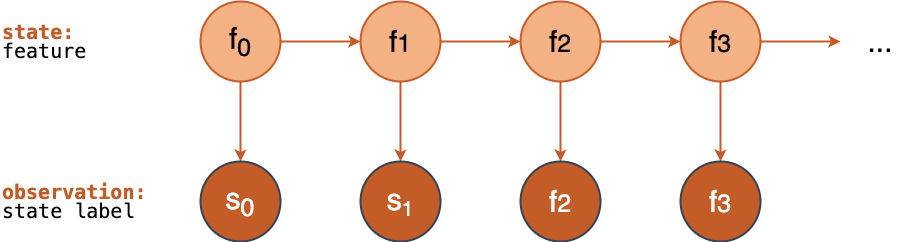
\includegraphics[width=0.8\linewidth]{figures/04_HMMmodel.png}
    \caption{Dynamic Graph Generation for Driver Behavior Recognition}
    \label{fig:HMMmodel}
\end{figure}


\section{Model architecture}

\subsection{JODIE: }
% what is JODIE
As is mentioned in chapter \ref{chapter:relatedwork}, the model \textit{JODIE} is a coupled recurrent neural network model that learns the embedding trajectories of users and items. Before we start our own contribution to the model, some introduction to the original model is necessary.

The model \textit{JODIE} is aimed at learning the embedding trajectories of users, denoted as $\mathbf{u(t)} \in \mathbb{R} ^n$ for each $u \in \mathcal{U}$ and item, denoted as $\mathbf{i(t)} \in \mathbb{R} ^n$ for each $i \in \mathcal{I} $, over a time interval $\forall t \in [0,T] $. These embeddings are derived from an ordered sequence of temporal user-item interactions $S_r=(u_r,i_r,t_r,\mathbb{f}_r)$, which indicates that an interaction $S_r$ involving a user $u_r \in \mathcal{U} $ and an item $i_r \in \mathcal{I} $ at time $t_r \in \mathbb{R} ^+$, in the period $0 < t_1 < t_2< \cdots  < T$. In our study, the \textit{user} corresponds to the driver, and the \textit{item} to the object of interaction. The process of interaction thus represents the driver’s behavior toward the object over time.

To encode both long-term stationary properties and the dynamic evolution of user-item interactions, the embedding contains \textbf{static and dynamic embeddings}. Static embeddings $\mathbf{\overline{u} } \in \mathbb{R} ^d \ \forall u \in \mathcal{U}$ and $\mathbf{\overline{i} } \in \mathbb{R} ^d \ \forall i \in \mathcal{I}$ keep constant over time, with one-hot vectors representation similar in LSTM\cite{zhu2017next} and TimeAware-LSTM\cite{baytas2017patient}.


The model could be separated into two parts: the \textbf{update operation} and the \textbf{projection operation}. In the update operation, the interaction $S=(u,i,t,f)$ between a user $u$ and item $i$ at time $t$ is used to generated their dynamic embeddings $\mathbf{u(t)}$ and $\mathbf{i(t)}$. Two recurrent neural networks RNNs are involved in this process, named $RNN_U$ and  $RNN_I$ . They recursively update the embeddings of the user and the item. 

% how do we change the loss function
% we training with the model adapted from JODIE




embedding function
$$ \mathbf{u(t)}=\sigma(W_1^u\mathbf{u(t^-)}+W_2^u\mathbf{i(t^-)}+W_3^uf+W^u_4 \Delta _u)$$
$$ \mathbf{i(t)}=\sigma(W_1^i\mathbf{i(t^-)}+W_2^i\mathbf{u(t^-)}+W_3^if+W^i_4 \Delta _i)$$

loss function(BCE)
$$L=-(j_{pos}\log{\tilde{j}}+j_{neg}log(1-\tilde{j}))$$

where

$$\tilde{j}(t+\Delta)=W_1\hat{u}(t+\delta)+W_2\bar{u}+W_3i(t+\Delta ^-)+W_4\bar{i}+B$$



\subsection{JODIE with state}
After comparing all the training results of the below models we would find that **JODIE** is one coming up with the best prediction. However, the model jodie still fail to predict the state of the predicted edge.
In my masterwork I would like to rewrite the embedding function and the loss function of **JODIE to make the state prediction possible.
- functions adapted in my work:

embedding function
$$ \mathbf{u(t)}=\sigma(W_1^u\mathbf{u(t^-)}+W_2^u\mathbf{i(t^-)}+W_3^uf+W^u_4s+W^u_5\Delta _u)$$
$$ \mathbf{i(t)}=\sigma(W_1^i\mathbf{i(t^-)}+W_2^i\mathbf{u(t^-)}+W_3^if+W^i_4s+W^u_5 \Delta _i)$$

we will change it from BCE to CE for predictiing state.

$$\tilde{j}(t+\Delta)=W_1\hat{u}(t+\delta)+W_2\bar{u}+W_3i(t+\Delta ^-)+W_4\bar{i}+W_5s+B$$

\subsection{abnormal detection}